\documentclass[11pt]{article}
\usepackage[margin=1in]{geometry}
\usepackage{graphicx,booktabs,amsmath,amssymb,url,microtype,xcolor,caption}
\usepackage[hidelinks]{hyperref}
\usepackage{times}
\captionsetup{font=small,labelfont=bf}
\newcommand{\code}[1]{\texttt{#1}}
\title{\textbf{Exhaustive AI-assisted review of SPM: eighty-three verified defects,\\ five fixes sent upstream, two merged and measured on open data}}
\author{Cynthia Condra\\ \small Unaffiliated \quad \texttt{cindy.krafft@gmail.com}}
\begin{document}
\maketitle

\begin{abstract}
SPM is among the most used neuroimaging packages and, like its peers, is large, old, mathematically dense, and read far less often than it is run. I asked an AI coding agent to read all of it adversarially, subsystem by subsystem, and to report nothing it could not reproduce by executing code. From the development source at commit \code{530ec52} (23 August 2026), divided into eleven subsystems, the review yielded 83 confirmed defects, each with file-and-line evidence and a numerical reproduction, and about 38 lower-confidence candidates recorded separately. The most reassuring result frames the rest: the standard fMRI general linear model, from \code{spm\_spm} through the T and F Euler-characteristic densities and both false-discovery procedures, was traced end to end and held. The defects sit in the tiers around that path. Five were ranked high priority by severity times reach and sent upstream as ordinary pull requests with issues carrying runnable reproductions: the $\chi^2$ Euler-characteristic densities in \code{spm\_ECdensity} use the wrong power of the threshold at dimensions two and three, so peak inference on $\chi^2$ maps is far too conservative and cluster inference far too liberal (a new unit test fails 12 of 23 assertions on the shipped code and none after the fix); the variational free energy in \code{spm\_nlsi\_GN} counts its log-determinant term $n_q$ times too often, which reaches DCM for evoked responses; \code{@meeg/badsamples} adds the peristimulus baseline twice when mapping artefact events to samples; \code{spm\_eeg\_downsample} stamps the requested rather than the achieved sampling rate; and \code{spm\_design\_contrasts} pads parametric-modulation columns without the basis-function factor. Within two days the maintainers merged the two M/EEG fixes; the other three are under review. To measure what the merged fixes mean in practice I ran SPM's own M/EEG code, executed in GNU Octave, on SPM's mismatch-negativity tutorial recording. Before the fix, every artefact window on epoched data sat 100\,ms late, so the detector excluded only 24\% of the artefact it had found and 71\% of what it excluded was clean; yet the final robust-averaged mismatch negativity moved by only 1.5\% RMS, because robust weighting cushions the mask. The sampling-rate defect, which fires only for the explicit \code{decimate} and \code{downsample} methods, reported a 915\,s recording as 781\,s and a 275\,ms mismatch-negativity peak at 235\,ms. Both reach corrections narrow the findings and are reported as such. The artefact-window fix was then measured where its geometry predicts the largest effect, on the open ERP CORE dataset (39 participants, two paradigms), with the same code and settings under both versions: on response-locked epochs beginning 600\,ms before the response, the shipped code placed 97\% of the detected artefact windows outside the epoch, so a rejection step that removes 51\% of trials after the fix removed 2\% before it, six participants with no clean error trials were silently given an error-related negativity, and the group ERN was $-10.4$\,$\mu$V before the fix against $-8.3$\,$\mu$V after (paired $p = 0.003$, $n = 30$); on stimulus-locked epochs with a 200\,ms baseline, and under robust averaging in either design, the change was small. The reviews, harnesses, patches, pipeline and results are public.
\end{abstract}

\section{Introduction}
Statistical Parametric Mapping \cite{friston2007} has carried a large share of published functional neuroimaging for three decades, and its M/EEG and dynamic causal modelling (DCM) branches carry much of the electrophysiology and effective-connectivity literature besides. The code base is excellent and heavily used, and both facts work against complete review: a routine that is correct for the inputs its author had in mind can be wrong for inputs that became common later, and a test suite cannot cover a regime nobody thought to test. When such a defect surfaces, as with cluster inference \cite{eklund2016}, it is treated as a singular event rather than as one instance of a class that could be searched for.

A companion paper reports the same method applied to AFNI, together with an end-to-end reanalysis of one merged fix on forty participants of an open dataset \cite{condra2026}. This paper is the SPM half, kept separate so that each package's findings can be read on their own terms. Its design has two deliberate features. The code review came first and any literature search second, so that findings were not filtered by what I expected to matter. And nothing was reported to the maintainers without a numerical reproduction and, where possible, a patch, so that the unit of output is a pull request rather than a suspicion. Section~\ref{sec:results} reports what was found, what was filed and what the maintainers merged. Section~\ref{sec:realdata} then takes the two merged fixes and asks what they change on SPM's own tutorial data, using SPM's own code.

\section{Methods}
\subsection{Exhaustive adversarial review}
An AI coding agent (Claude, Anthropic) worked in a sandboxed environment with the SPM source checked out (\code{spm/spm} development version at \code{530ec52}, 23 August 2026), a C compiler, Python with NumPy and SciPy, and later GNU Octave. The source was divided into eleven subsystems, each read in full by a separate agent with an adversarial brief: for every routine, what inputs are legal but unanticipated, what happens at boundaries and at zero, where do numeric types and index bases change, where is a convention assumed rather than checked. The subsystems were the statistical distribution library; random field theory and the results machinery; the GLM estimation core including ReML; spatial preprocessing; image and file I/O; the C and MEX sources; DCM and Bayesian inversion; numeric and mesh utilities; M/EEG processing including the \code{@meeg} object; the spatial toolboxes (FieldMap, DARTEL, Shoot, Longitudinal, OldNorm, OldSeg, Spatial); and the active-inference code (\code{spm\_MDP\_*} and its tensor helpers). A human directed the agent at the level of package, subsystem and which candidates to pursue; the agent wrote the reviews, harnesses and patches. Every candidate was recorded with file and line evidence, and code paths that were checked and found correct were recorded with the same care.

\subsection{Verification by execution}
No candidate was reported without execution of one of three kinds: transcribing the routine faithfully to Python, idiosyncrasies included, and testing the transcription against NumPy, SciPy, closed forms or Monte Carlo; checking a claimed identity numerically (for the Euler-characteristic densities, that $\chi^2_1 = Z^2$ and $\chi^2_\nu = \nu F(\nu,\infty)$, and for the Wishart divergence, a Monte-Carlo estimate of the true Kullback--Leibler value); or running the shipped MATLAB code itself. The third kind became possible once SPM was built for GNU Octave 8.4 with \code{make PLATFORM=octave}. Two of SPM's dependencies had to be replaced for that: FieldTrip's 24-bit BDF reader, which ships only as a MEX binary, was replaced by an equivalent pure-MATLAB decoder verified against MNE-Python's independent decode to four decimals, and a handful of MATLAB-only string helpers were shimmed. Candidates that did not survive execution were recorded as plausible, not confirmed, and are not counted among the 83.

\subsection{Triage and upstream filing}
Confirmed findings were ranked by severity times how often the code path runs in real pipelines, with silent failure weighted above a crash, into three tiers. The top tier was patched on a fork as one branch per fix, each with a commit message and, for the first, a new unit test in the repository's own \code{matlab.unittest} pattern. Following SPM's contributing guide, each fix was filed as a GitHub issue stating expected and actual behaviour with a runnable MATLAB snippet, paired with a pull request. Each pull request states what testing was done and what was not: the $\chi^2$ fix and the two M/EEG fixes were executed in Octave, the other two were verified by transcription and tracing only. The maintainers' review is the adjudication.

\subsection{Literature exposure, assessed afterwards}
Exposure was assessed only after the review and only for the top tier, by anchoring each finding to the methods papers that document the affected machinery, rather than by a per-paper join of the kind the AFNI companion performs for one finding. That join for SPM is future work and its absence is a stated limitation.

\subsection{Measuring the merged fixes on SPM's tutorial data}
\label{sec:mmnmethods}
\paragraph{Data.} SPM's mismatch-negativity (MMN) tutorial recording (\code{eeg\_mmn/subject1.bdf}): one participant, 128-channel Biosemi EEG at 512\,Hz, 915\,s, passive auditory oddball with 480 standards and 120 deviants \cite{garrido2007,naatanen2007}.

\paragraph{Artefact-window defect (\code{@meeg/badsamples}, PR 163).} SPM's own ``advanced artefact removal'' chapter for this dataset was run with the real SPM functions in Octave: downsample to 200\,Hz, band-pass 0.5--30\,Hz, epoch $-100$ to 400\,ms with baseline correction, artefact detection in \code{mark} mode (z-scored-difference detector, 100\,ms excision window, bad-channel threshold 1), then robust averaging with ``remove bad data'' on, and MMN as deviant minus standard. The pipeline was run twice, with \code{badsamples.m} at \code{530ec52} and at upstream \code{main} after the merge; everything else was identical. The two bad-sample masks were compared directly, and the two MMN waveforms by global field power.

\paragraph{Sampling-rate defect (\code{spm\_eeg\_downsample}, PR 165).} The recording was downsampled from 512 to a requested 200\,Hz with \code{method = 'decimate'} using the real \code{spm\_eeg\_downsample} in Octave, before and after the fix, and the stamped rate and the reported time of the last sample were read from the resulting object. The consequence for the MMN was computed by a Python transcription of the same arithmetic (decimation by the rounded factor, 0.5--30\,Hz, average reference, epoch $-100$ to 400\,ms): the true waveform was placed on the true time axis and on the axis the pre-fix stamp implies. The default \code{resample} method and the no-toolbox \code{fft} fallback are exact, so the defect was also confirmed \emph{not} to fire there.

\subsection{Measuring the artefact-window fix on ERP CORE}
\label{sec:erpmethods}
The MMN measurement is one participant, a 100\,ms baseline and a workflow with a second safety net. The defect's shift equals the distance from epoch start to time zero, so its consequences should scale with that distance, and they should be uncushioned wherever the mask is consumed directly. To test both predictions on an open multi-participant dataset I used ERP CORE \cite{kappenman2021}: 40 neurotypical adults, Biosemi ActiveTwo, 30 scalp channels and three EOG channels at 1024\,Hz, seven paradigms with published bin definitions and measurement windows. Two paradigms were chosen for their epoch geometry: the active visual oddball (P3), stimulus-locked, epoch $-200$ to 800\,ms, measure target minus standard at Pz over 300--600\,ms; and the flankers task (ERN), response-locked, epoch $-600$ to 400\,ms, measure error minus correct at FCz over 0--100\,ms. The OSF folders hold raw files for 39 participants per task; all 39 were processed.

\paragraph{Pipeline.} Real SPM functions executed in Octave. The build-independent stage, run once per participant: conversion from EEGLAB format; ERP CORE's 26\,ms stimulus-code correction; re-referencing to the P9/P10 average with bipolar VEOG and HEOG, as in ERP CORE; resampling to 256\,Hz with the exact \code{resample} method, so the sampling-rate defect cannot enter; 0.1\,Hz high-pass and 30\,Hz low-pass; epoching with ERP CORE's bin definitions (P3: stimuli followed by a correct response within 200--1000\,ms; ERN: responses preceded by a flanker stimulus within 200--1000\,ms) and baselines ($-200$ to 0\,ms; $-400$ to $-200$\,ms). The build-dependent stage, run on the same epoched file once with \code{badsamples.m} at \code{530ec52} and once at upstream \code{main} after PR 163: \code{spm\_eeg\_artefact} in \code{mark} mode (channel threshold 100\,$\mu$V, 200\,ms excision window, EEG and EOG channels, bad-channel threshold 0.2), then the two consumers of the resulting mask, (i) \code{spm\_eeg\_artefact} in \code{reject} mode with the \code{events} plugin, which rejects a trial if any channel carries a marked sample, followed by a plain average, and (ii) robust averaging with \emph{remove bad data}. No ocular correction was applied; this is the threshold-only pipeline SPM's manual chapters use, and it is harsh on blink-heavy participants under either build, which the results state. The two builds see identical detector output; only the reading of it differs.

\paragraph{Analysis.} Per participant and build: the bad-sample mask, its overlap with the fixed mask (which reproduces the detector's intent, as verified on the MMN data), the share of the detector's windows the shift places entirely outside the epoch, channels classified bad, trials rejected, trials retained per condition, and the ERP measure under each consumer. Group level: the measure before against after the fix by paired $t$-test, restricted to participants retaining at least six trials of the condition of interest under both builds, since a participant with no error trials has no ERN under a correctly working rejection step. One Octave compatibility patch, identical in both trees, made \code{spm\_robust\_average}'s median helper return NaN for an all-NaN column as MATLAB does.

\section{Results: what was found and what was merged}
\label{sec:results}
\subsection{Counts and the path that held}
The review produced 83 confirmed defects, each producing wrong numbers, wrong geometry, a crash or silent data corruption on a concrete input, plus about 38 plausible candidates tracked in the component reviews. Triage placed 5 in the high-priority tier, 15 in the medium tier and 63 in the low tier. Against them stand the paths that were checked and held: the Z, T and F Euler-characteristic densities, \code{spm\_P\_RF} in both its unified and Poisson-clumping forms, both FDR procedures, Bonferroni, \code{spm\_resels} and \code{spm\_est\_smoothness}; the GLM core (\code{spm\_spm}'s whitening and degrees-of-freedom machinery, the Satterthwaite trace identities, the ReML gradients and curvatures, \code{spm\_hrf}, filter construction, microtime onsets); the NIfTI quaternion round-trip to $3\times10^{-12}$ over 20{,}000 rotations and every 0-based/1-based voxel convention traced; \code{spm\_matrix} and \code{spm\_imatrix} including negative determinants; the DCM hemodynamic equations, Jacobians, \code{spm\_BMS} and the Bayesian model-reduction closed form; the mainstream robust-averaging routine \code{spm\_robust\_average}; and the \code{spm\_dot} and \code{spm\_kron} tensor conventions against \code{einsum}. A standard fMRI analysis with the default HRF, realign, coregister, normalise, smooth, T and F contrasts, and RFT or FDR thresholding runs on verified code from end to end. The defects cluster in the tiers out from it: specific statistic types, optional features, particular toolboxes, rare formats and edge cases.

\subsection{The high-priority tier}
Table~\ref{tab:tier1} lists the five findings sent upstream and their status. Each is described briefly here; the component reviews hold the file-and-line evidence.

\begin{table}[t]
\centering\small
\caption{The five high-priority findings, their fixes, and upstream status as of 3 September 2026. Each pull request is paired with an issue carrying a runnable reproduction. ``Executed'' means the fix was run against the real SPM code in Octave; the others were verified by transcription and tracing, which each pull request states.}
\label{tab:tier1}
\begin{tabular}{@{}lp{6.9cm}lll@{}}
\toprule
 & Defect & Verified & Issue / PR & Status \\
\midrule
SP1 & \code{spm\_ECdensity}: $\chi^2$ EC densities use $t^{(\nu-1)/2}$ at every order where Worsley's densities need $t^{(\nu-d)/2}$; 2-D density inflated by $\sqrt t$, 3-D by $t$ & executed, unit test & 158 / 159 & open \\
SP2 & \code{spm\_nlsi\_GN}: free energy applies the $n_q$ factor to an already Kronecker-expanded precision, overcounting the log-determinant $n_q$-fold; the M-step gradient is that of the corrected term & traced & 160 / 161 & open \\
SP3 & \code{@meeg/badsamples}: peristimulus baseline added twice when mapping artefact events to samples; every window on epoched data shifted by the baseline & executed, real data & 162 / 163 & merged 2 Sep \\
SP4 & \code{spm\_eeg\_downsample}: achieved rate computed and printed, requested rate stored & executed, real data & 164 / 165 & merged 2 Sep \\
SP5 & \code{spm\_design\_contrasts}: parametric-modulation padding uses $\sum h$ columns where the design carries $\sum h \cdot n_{\mathrm{bases}}$; automatic factorial contrasts slide onto the wrong regressors when derivatives are on & numerically & 167 / 168 & open \\
\bottomrule
\end{tabular}
\end{table}

\paragraph{SP1: $\chi^2$ Euler-characteristic densities.} Random field theory gives the expected Euler characteristic of an excursion set as a sum over dimensions of resel counts times EC densities \cite{worsley1994}. In \code{spm\_ECdensity} the $\chi^2$ branch computes a single factor $t^{(\nu-1)/2}$ and reuses it at orders two and three, where the densities need $t^{(\nu-2)/2}$ and $t^{(\nu-3)/2}$; the 2-D density is therefore inflated by $\sqrt t$ and the 3-D density by $t$ (Fig.~\ref{fig:findings}A). Three independent checks agree: a transcription cross-checked through the identities $\chi^2_1 = Z^2$ and $\chi^2_\nu = \nu F(\nu,\infty)$; a Monte-Carlo simulation of smooth $\chi^2_4$ fields on a $256^2$ torus (300 realisations, FWHM 8 pixels), where the empirical expected Euler characteristic at thresholds 12, 16 and 20 was 59.5, 15.1 and 3.2 against 60.5, 15.8 and 3.5 from the corrected formula and 209.5, 63.1 and 15.6 from the shipped one; and, after patching, execution of the real MATLAB code in Octave, where the new \code{tests/test\_spm\_ECdensity.m} fails 12 of 23 assertions on the shipped code and none on the fix, with the untouched Z, T and F branches bit-identical. The function had no test before. End to end, on a whole-brain $\chi^2_{10}$ map at threshold 40, \code{spm\_P\_RF} gives a peak family-wise $p$ of 1.000 where the correct value is 0.380, and a cluster-extent $p$ of $10^{-9}$ where the correct value is 0.050: inference is invalid in both directions. Reach is narrow. $\chi^2$ statistic images are rare in applied work, the standard conjunction analysis uses the minimum statistic and is not exposed, and no high-citation empirical SPM\{$\chi^2$\} paper was found. That is the honest reason a defect this severe ranks with, and not above, the rest of the tier.

\paragraph{SP2: free energy in \code{spm\_nlsi\_GN}.} The variational free energy that DCM reports and ranks models by includes a term $\tfrac12\log|\Sigma^{-1}|$ in the data precision. At line 500 the precision has already been expanded across the $n_q$ error-covariance blocks, and the code multiplies its log-determinant by $n_q$ once more, so the term is $n_q^2/2$ times the block value rather than $n_q/2$. The M-step gradient a few lines away uses $n_y/2$, the derivative of the corrected term, so objective and gradient currently disagree. Inversions with a single block, which includes DCM for fMRI, are unaffected. DCM for evoked and induced responses, where $n_q$ is channels times trials, has the hyperparameter-dependent part of $F$ inflated $n_q$-fold, which can alter model rankings, the primary output of that method \cite{david2006,garrido2007}. This finding is confirmed by internal inconsistency and transcription; it has not been executed in MATLAB, which the pull request states.

\paragraph{SP3: artefact windows on epoched data.} SPM's artefact detectors write event times relative to trial onset without the peristimulus offset \code{timeOnset}, because the two occurrences cancel in their arithmetic. The reader \code{badsamples} then adds \code{time(this)}, which includes it. Every bad-sample window on epoched data is therefore shifted late by the baseline length: 20 samples for a 100\,ms baseline at 200\,Hz (Fig.~\ref{fig:findings}B). Clean data are excluded and artefact partially retained, silently. The shift reaches the \code{mark} artefact mode, where bad channels are classified by the fraction of bad samples, the ``remove bad data'' option of robust averaging, cross-frequency-coupling weights and other consumers of the mask on epoched data. It does not reach the default \code{reject} mode, which never calls \code{badsamples}, nor continuous data, where the offset is zero. The machinery is that documented by the SPM8 M/EEG reference paper \cite{litvak2011}. Merged as PR 163 and measured in Section~\ref{sec:realdata}.

\paragraph{SP4: the stamped sampling rate.} \code{spm\_eeg\_downsample} computes the achieved rate and prints it, then stores the requested one. The two differ only when the user explicitly selects \code{decimate} or \code{downsample} with a non-integer ratio, because FieldTrip's \code{ft\_preproc\_resample} then rounds the factor; the default \code{resample} method and the no-toolbox \code{fft} fallback are exact. That is narrower than the audit's first framing, and it is recorded. Merged as PR 165 and measured in Section~\ref{sec:realdata}.

\paragraph{SP5: parametric modulators with basis-function expansion.} When automatic factorial contrasts are built, \code{spm\_design\_contrasts} skips the parametric-modulation columns by inserting $\sum h$ zeros, where $h$ counts the modulators; but every modulator column is convolved with all basis functions in \code{spm\_Volterra}, so the design carries $\sum h \cdot n_{\mathrm{bases}}$ such columns. Whenever temporal or dispersion derivatives are on and modulators are present, the contrast matrix is misaligned from the first modulated condition onward, and the trailing zero-pad hides the mismatch, so wrong F and T maps arrive without an error. The combination of factorial design and derivatives is the one popularised by \cite{henson2002}; whether specific studies also used modulators with automatic contrasts is unverified. Confirmed numerically on a constructed design; not executed in MATLAB.

\subsection{The medium and low tiers}
The fifteen medium-tier findings are common features with a conditional trigger, or important narrower methods. Representative examples: \code{spm\_dicom\_convert} pairs pixel spacing with the wrong direction cosines, swapping in-plane voxel sizes for non-square pixels (the spectroscopy path swaps them back with a comment saying ``for some reason''); \code{spm\_file\_merge} has a sign error that clips negative intensities when merging 3-D integer volumes into 4-D; \code{spm\_preproc\_write8} returns warped and modulated tissue classes in swapped slots; \code{spm\_dcm\_peb} nests its convergence test inside \code{if verbose}, so with printing off the parametric empirical Bayes routine \cite{friston2016} always runs 64 iterations and results depend on a display preference; \code{spm\_kl\_wishart} takes the expectation of $\log|X|$ under the wrong distribution (Monte-Carlo true divergence 6.560, coded 7.681, corrected 6.559) and \code{spm\_lg\_gamma} sums ascending arguments where the multivariate gamma descends; the windowed Fourier transform pair uses the conjugate transpose where it needs the plain one and does not round-trip; \code{spm\_powell}'s bracket clamp has the wrong sign for descending line searches, degrading mutual-information coregistration; the FieldMap FFT smoothing grid is half a voxel off-centre on odd dimensions; \code{spm\_robust\_glm} multiplies residuals by leverage instead of dividing by $\sqrt{1-h}$, so it never down-weights anything, though only the mixture toolbox calls it; and in the active-inference engine \cite{friston2017} the B-novelty term indexes the action dimension with the policy index and \code{spm\_MDP\_MI}'s Dirichlet gradient is 50--100\% off with the wrong sign pattern, which steers structure learning by Bayesian model reduction \cite{smith2020} the wrong way. Five further findings are loud crashes on documented but rarely used modes. The 63 low-tier findings are distribution edge cases, rare datatypes and formats, latent defects with no live caller, C/MEX boundary conditions, minor I/O and tabular issues, mesh and numeric utilities, M/EEG convention slips such as swapped sine and cosine phase regressors, and preprocessing minutiae, all listed with file and line in the repository.

\section{Results: the two merged fixes on SPM's own data}
\label{sec:realdata}
\subsection{Artefact windows: a mask that was mostly wrong, and an average that barely moved}
Table~\ref{tab:sp3} gives the comparison. On trial 5 the detector recorded an artefact beginning at epoch sample 30; the shipped reader marked samples 51 to 77 and the fixed reader 31 to 57 (Fig.~\ref{fig:findings}B). Across the 316 channel-by-trial bad runs present under both versions the median onset shift was exactly 20 samples, the 100\,ms baseline. The two masks overlapped with a Jaccard index of 0.15. Of the samples the detector had actually flagged, the shipped code excluded 24\%; of the samples it excluded, 71\% were clean. One hundred bad runs were truncated at the epoch end under the shipped code against 37 after the fix, so ten trials' artefacts were pushed off the edge of the epoch and lost entirely, and the total count of marked samples fell 16\%, which is the quantity \code{mark} mode thresholds when it classifies channels as bad.

The final waveform hardly changed (Fig.~\ref{fig:findings}C). The robust-averaged MMN peaked at 255\,ms under both versions, with global field power 2.771 against 2.778\,$\mu$V and the same largest channel at $-10.91\,\mu$V; the largest difference at any channel and time was 0.37\,$\mu$V, and the RMS difference over 100--300\,ms was 0.044\,$\mu$V against an MMN RMS of 2.94\,$\mu$V, about 1.5\%. The reason is that in this workflow the mask is redundant with the robust weights, which already down-weight the outlying samples the mask was meant to remove, whether or not the mask lands on them; only 84 to 94 of 600 trials carried any detected artefact, and blinks in a passive oddball are not time-locked to the deviants, so the misplaced exclusions do not bias the average systematically. Where the mask is consumed directly, in bad-channel and bad-trial classification and in the other mask consumers named above, there is no such cushion.

\begin{table}[t]
\centering\small
\caption{The artefact-window fix on SPM's MMN tutorial recording: SPM's own mark-mode plus robust-averaging chapter, executed with the real code in Octave, with \code{badsamples.m} before and after PR 163 and nothing else changed. 600 epochs of 101 samples at 200\,Hz, baseline 20 samples.}
\label{tab:sp3}
\begin{tabular}{@{}lcc@{}}
\toprule
 & Before fix & After fix \\
\midrule
Trial 5: detector wrote artefact at sample 30; samples marked & 51--77 & 31--57 \\
Median onset shift over 316 shared bad runs & 20 samples (100\,ms) & \\
Bad samples marked in total & 7{,}584 & 9{,}017 \\
Trials with any bad sample & 84 & 94 \\
Bad runs truncated at the epoch end & 100 & 37 \\
Jaccard overlap of the two masks & \multicolumn{2}{c}{0.151} \\
Share of detected artefact samples actually excluded & 24.2\% & 100\% \\
Share of excluded samples that were clean & 71.2\% & 0\% \\
\midrule
Robust-averaged MMN: global field power peak & 255\,ms (2.771\,$\mu$V) & 255\,ms (2.778\,$\mu$V) \\
Largest channel at peak (A14) & $-10.91\,\mu$V & $-10.91\,\mu$V \\
Largest difference, any channel and time & \multicolumn{2}{c}{0.37\,$\mu$V at 300\,ms} \\
RMS difference over 100--300\,ms (MMN RMS 2.94\,$\mu$V) & \multicolumn{2}{c}{0.044\,$\mu$V (1.5\%)} \\
\bottomrule
\end{tabular}
\end{table}

\subsection{Sampling rate: the right number printed, the wrong one stored}
Requesting 200\,Hz from 512\,Hz with \code{decimate} rounds the factor to 3, so the data are really at $512/3 = 170.667$\,Hz. Both versions print ``170.7\,Hz''. The shipped version stores 200\,Hz, so the object reports its last sample at 780.8\,s of a 915.0\,s recording; the fixed version stores 170.7\,Hz and reports 914.8\,s (Table~\ref{tab:sp4}). Every time value derived from the file is 14.7\% too small under the shipped stamp. On the MMN this moves the global-field-power peak from its true 275.4\,ms to a reported 235.0\,ms (Fig.~\ref{fig:findings}D), and silently mis-cuts every user-specified window: a requested $-100$ to 400\,ms epoch covers $-85$ to 341\,ms of real time, the baseline $-85$ to 0\,ms, and a 100--250\,ms MMN window 85--213\,ms. The residual 0.02\% between 170.7 and 170.667\,Hz, which the display rounding introduced and the fix inherits, is outside the fix's scope and noted in the pull request.

\begin{table}[t]
\centering\small
\caption{The sampling-rate fix: the real \code{spm\_eeg\_downsample} in Octave, 512\,Hz to a requested 200\,Hz with \code{method = 'decimate'}, before and after PR 165. The MMN rows come from a Python transcription of the same arithmetic on the same recording.}
\label{tab:sp4}
\begin{tabular}{@{}lcc@{}}
\toprule
 & Before fix & After fix \\
\midrule
Printed resampling frequency & 170.7\,Hz & 170.7\,Hz \\
Stored \code{fsample} & 200.0\,Hz & 170.7\,Hz \\
Reported time of last sample (true 914.994\,s) & 780.795\,s & 914.815\,s \\
Reported MMN peak latency (true 275.4\,ms) & 235.0\,ms & 275.4\,ms \\
Real-time extent of a requested $-100$ to 400\,ms epoch & $-85$ to 341\,ms & $-100$ to 400\,ms \\
\bottomrule
\end{tabular}
\end{table}

\begin{figure}[p]
\centering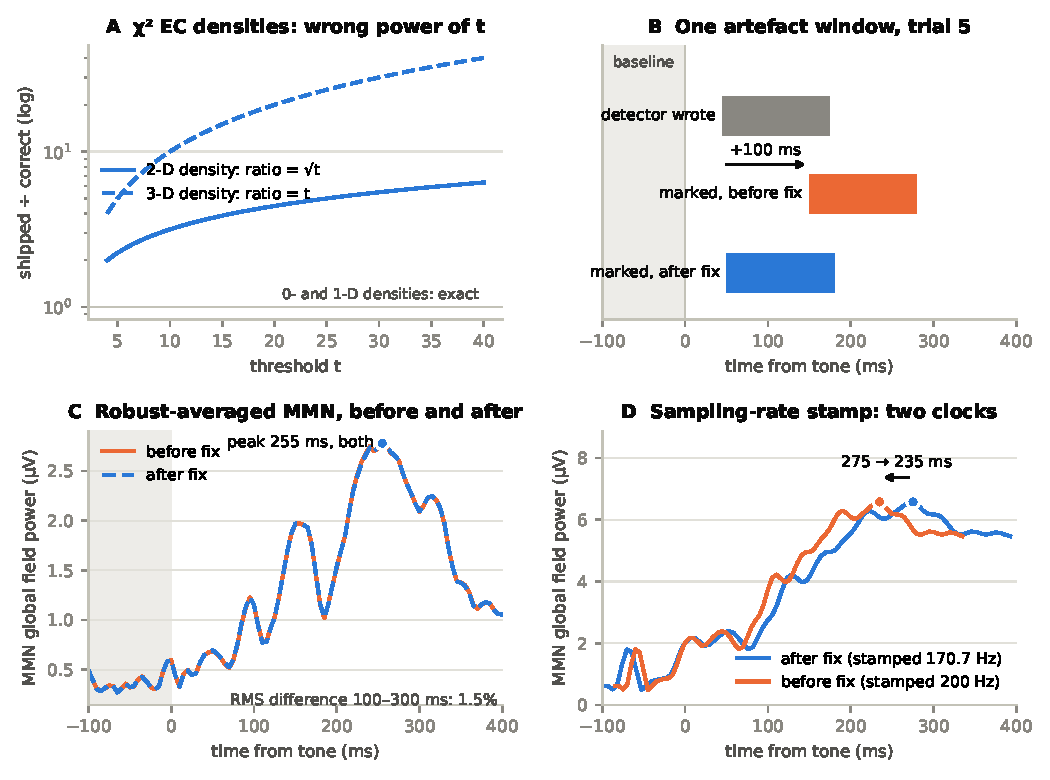
\includegraphics[width=\textwidth]{figures/findings.pdf}
\caption{\textbf{Two of the five high-priority defects, and the two merged ones on SPM's own data.} \textbf{A}, The $\chi^2$ Euler-characteristic densities in \code{spm\_ECdensity}: ratio of shipped to correct density against threshold, for the 2-D ($\sqrt t$) and 3-D ($t$) orders; orders zero and one are exact. \textbf{B}, One artefact on trial 5 of the MMN tutorial recording: the window the detector recorded (grey), the samples the shipped \code{badsamples} marked (orange) and the samples the fixed version marks (blue). The shift is the 100\,ms baseline. \textbf{C}, Global field power of the robust-averaged MMN from SPM's own artefact-removal chapter, with \code{badsamples} before (orange) and after (blue) the fix; the mask changed wholesale, the average by 1.5\%. \textbf{D}, The MMN from the same recording decimated from 512 to a nominal 200\,Hz, placed on the true time axis (blue, the rate the fixed \code{spm\_eeg\_downsample} stores) and on the axis the shipped stamp implies (orange); the true 275\,ms peak is reported at 235\,ms. Panels B and C use the real SPM code in Octave; panel D uses a Python transcription of the decimation arithmetic.}
\label{fig:findings}
\end{figure}

\subsection{The artefact-window fix on 39 ERP CORE participants}
\label{sec:erpcore}
Table~\ref{tab:erpcore} and Figure~\ref{fig:erpcore} give the comparison. The geometry prediction held exactly. In the stimulus-locked P3 design the 200\,ms shift pushed 15\% of the detector's windows out of the epoch and the shipped code excluded a median 30\% of the artefact samples it had found. In the response-locked ERN design the 600\,ms shift pushed 97\% of the windows out, because blinks cluster after the response, at 600--1000\,ms into the epoch, and are read back 600\,ms later, off its end; the shipped code excluded a median 0.5\% of the artefact it had found, and its mask overlapped the correct one with a Jaccard index of 0.005. Everything built on that mask behaved as if the artefact step had not run: no channel was classified bad in any participant before the fix against 16 channels in 8 participants after it, and a rejection step that removes 51\% of all trials after the fix removed 2\% before it.

\begin{table}[t]
\centering\small
\caption{The artefact-window fix on ERP CORE, 39 participants per paradigm, real SPM code in Octave with \code{badsamples.m} before and after PR 163 and nothing else changed. Group rows use participants with at least six trials of the condition of interest under both builds. Medians are over participants.}
\label{tab:erpcore}
\begin{tabular}{@{}lcc@{}}
\toprule
 & P3 (shift 200\,ms) & ERN (shift 600\,ms) \\
\midrule
Detector windows written & 20{,}648 & 39{,}155 \\
Windows placed entirely outside the epoch before the fix & 15\% & 97\% \\
Share of true artefact samples excluded before the fix (median) & 30\% & 0.5\% \\
Share of pre-fix exclusions that were clean (median) & 33\% & 17\% \\
Channels classified bad, before / after & 5 / 20 & 0 / 16 \\
Trials rejected, before / after & 50\% / 56\% & 2\% / 51\% \\
Participants left with no trials of interest, before / after & 1 / 3 & 0 / 6 \\
\midrule
\multicolumn{3}{@{}l}{\emph{Event-based rejection, plain average}} \\
Participants analysed & 24 & 30 \\
Group mean, before / after & 7.6 / 7.4\,$\mu$V & $-10.4$ / $-8.3$\,$\mu$V \\
Paired $t$, $p$ & 1.10, 0.28 & $-3.23$, 0.003 \\
Correlation of per-participant values & 0.99 & 0.76 \\
Median absolute change per participant & 0.29\,$\mu$V (6\%) & 2.1\,$\mu$V (24\%) \\
Participants changed by more than 10\% & 11 of 24 & 22 of 30 \\
\midrule
\multicolumn{3}{@{}l}{\emph{Robust averaging with remove bad data}} \\
Group mean, before / after & 5.61 / 5.60\,$\mu$V & $-9.46$ / $-9.31$\,$\mu$V \\
Correlation of per-participant values & 0.9997 & 0.993 \\
Participants changed by more than 1\,$\mu$V & 0 & 1 \\
\bottomrule
\end{tabular}
\end{table}

\begin{figure}[p]
\centering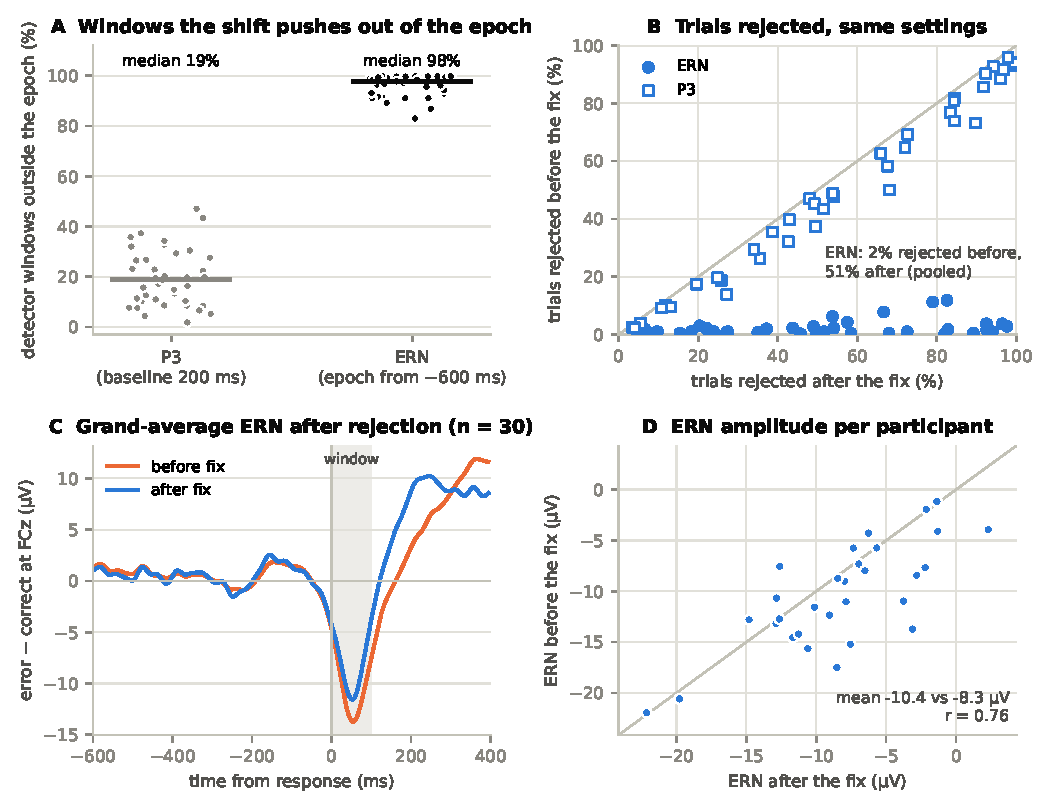
\includegraphics[width=\textwidth]{figures/erpcore.pdf}
\caption{\textbf{The artefact-window fix on ERP CORE.} \textbf{A}, Share of each participant's detector windows that the shipped \code{badsamples} places entirely outside the epoch, for the stimulus-locked P3 (200\,ms shift) and the response-locked ERN (600\,ms shift); bars are medians. \textbf{B}, Trials rejected per participant by the same event-based rejection settings under the shipped code (vertical) and the fixed code (horizontal). \textbf{C}, Grand-average error-minus-correct waveform at FCz after rejection and plain averaging, shipped (orange) and fixed (blue), over the 30 participants with at least six error trials under both; shaded, the 0--100\,ms measurement window. \textbf{D}, The per-participant ERN measure under the two builds.}
\label{fig:erpcore}
\end{figure}

The downstream numbers followed. Under the shipped code the same settings retained 98\% of ERN trials, and the grand-average ERN over the 30 participants analysed was 26\% larger than under the fixed code, $-10.4$ against $-8.3$\,$\mu$V, with a broader waveform and a delayed error positivity (Fig.~\ref{fig:erpcore}C), consistent with blink and movement artefact retained in the error trials. The paired difference is reliable ($t_{29} = -3.23$, $p = 0.003$); per-participant values correlated 0.76; the median participant changed by 2.1\,$\mu$V, a quarter of their ERN. Six participants who have no artefact-free error trials at this threshold, and whom the fixed code correctly leaves without an ERN, were silently given one by the shipped code. The effect is not one of significance, since the ERN is strongly present under both builds; what changed is its size, its shape, and which participants contribute. In the P3 design the two builds agreed closely (correlation 0.99, median change 6\%, no group shift), and under robust averaging with remove-bad-data both designs agreed almost perfectly (correlations 0.9997 and 0.993), as on the MMN data: the samples the mask fails to remove are the ones the robust weights down-weight anyway.

\section{Discussion}
\paragraph{What the review establishes.} SPM's most travelled path is sound. The defects that were found live one step out from it, in $\chi^2$ inference, in the M/EEG artefact and resampling machinery, in DCM for electrophysiology, in automatic contrasts with derivatives, and further out still in toolboxes and formats. Two of the five fixes at the top of the list were merged within two days of filing, each with a reproduction the maintainer could run, and three are under review; the deliverable is the merged code, and the maintainers' reading of the rest, not mine, is what will make it trustworthy.

\paragraph{Severity and reach are different axes, and both were measured.} The $\chi^2$ defect is the most severe finding here, invalidating inference in both directions, and it is the one with the thinnest exposure. The artefact-window defect corrupts its mask wholesale; on the canonical MMN pipeline the corruption is absorbed by a second safety net, and on response-locked or long-baseline epochs consumed without one it silently disables the artefact step and moves a group ERP by a quarter. The sampling-rate defect fires only when a user picks a non-default method with a non-integer ratio, and when it fires it is not subtle. In each case the measurement narrowed the finding relative to the audit's first framing, and the narrowing is recorded next to the finding. That is what verification is for: it moves candidates out of the confirmed set as readily as it moves them in.

\paragraph{Why the defects survived.} Each routine was correct for the data its author tested it on. The $\chi^2$ branch had no unit test at all, and a T or F user never exercises it. The artefact detector and the artefact reader each handled the baseline consistently with themselves, and only disagreed with each other, on a path the default mode does not take. The resampler printed the right number. No user could see a defect whose signature is ``artefact windows 100\,ms late'' or ``a peak 40\,ms early on a file that says 200\,Hz.'' This is the general shape of the findings: not carelessness, but the combinatorics of a large, old code base and evolving conventions, which no team can read exhaustively with the question ``what if the offset is nonzero, or the ratio is not an integer, or there are two basis functions'' in mind for every line. A machine can now ask that question of every line cheaply, and the answers arrive in the form maintainers already accept.

\paragraph{Limitations.} ``Confirmed'' means traced end to end and reproduced as stated, not adjudicated by the maintainers; where they disagree, their reading wins. SPM was executed in GNU Octave, not MATLAB, with two dependencies replaced; the replaced reader was verified against an independent decoder, and the MEX files were built from SPM's own sources, but a MATLAB-specific difference cannot be excluded. The MMN measurement is one participant and one pipeline, chosen because it is the pipeline SPM's own documentation teaches for this recording; the ERP CORE measurement is 39 participants but a threshold-only pipeline without ocular correction, which rejects half of all ERN trials once it works as specified, so the group values reported are build-against-build comparisons and not estimates of the published ERP CORE effects. SP2 and SP5 have not been executed in MATLAB and their pull requests say so. The FieldMap review is partial. Exposure was assessed at the level of methods papers only; the per-study join that the AFNI companion performs for one finding has not been done for SPM, so this paper makes no claim about any individual published result. And a review of this kind is exhaustive with respect to what the agents read and checked, which is recorded, not with respect to every defect the code contains.

\section*{Data and code availability}
The eleven component reviews, every verification harness (Python transcriptions, the $\chi^2$ Monte Carlo, the Octave regression and unit-test driver), the real-data pipelines (\path{audits/spm/reproductions/mmn_realdata/}: \code{sp3\_pipeline.m}, \code{sp3\_compare.py}, \code{sp4\_demo.py}, the Octave shims, run logs and result notes; \path{audits/spm/reproductions/erpcore_realdata/}: the ERP CORE pipeline, per-participant tables, run logs and the figure script), the filing kit with issue and pull-request texts, and the script that draws Figure~\ref{fig:findings} are at \url{https://github.com/cindykrafft/research-software-audit}. The fixes are on \url{https://github.com/cindykrafft/spm} as one branch per fix, based on \code{spm/spm} at \code{530ec52}. Upstream: issues 158, 160, 162, 164 and 167 and pull requests 159, 161, 163, 165 and 168 at \url{https://github.com/spm/spm}; 163 and 165 are merged. The recordings are SPM's public MMN tutorial dataset and ERP CORE (OSF \code{thsqg}).

\section*{Disclosure of AI use}
The code reviews, harnesses, patches and the Octave build described here were produced by an AI coding agent (Claude, Anthropic) operating under the author's direction; every reported finding was verified by executing code, and every upstream filing was reviewed by the author before submission. The same system assisted in drafting this manuscript and produced its figure from the checked-in results. The author has no financial interest in any software named.

\begin{thebibliography}{99}
\bibitem{friston2007} Friston KJ, Ashburner J, Kiebel S, Nichols T, Penny W (eds). \emph{Statistical Parametric Mapping: The Analysis of Functional Brain Images}. Academic Press (2007).
\bibitem{eklund2016} Eklund A, Nichols TE, Knutsson H. Cluster failure: why fMRI inferences for spatial extent have inflated false-positive rates. \emph{Proc Natl Acad Sci USA} 113:7900--7905 (2016).
\bibitem{condra2026} Condra C. Exhaustive AI-assisted review of research software finds merged, verified defects in AFNI, and a thirteen-year-old error in regional homogeneity changes a group result. Preprint (2026); source in the same repository, \code{preprint/}.
\bibitem{worsley1994} Worsley KJ. Local maxima and the expected Euler characteristic of excursion sets of $\chi^2$, $F$ and $t$ fields. \emph{Adv Appl Probab} 26:13--42 (1994).
\bibitem{david2006} David O, Kiebel SJ, Harrison LM, Mattout J, Kilner JM, Friston KJ. Dynamic causal modeling of evoked responses in EEG and MEG. \emph{NeuroImage} 30:1255--1272 (2006).
\bibitem{garrido2007} Garrido MI, Kilner JM, Kiebel SJ, Friston KJ. Evoked brain responses are generated by feedback loops. \emph{Proc Natl Acad Sci USA} 104:20961--20966 (2007).
\bibitem{naatanen2007} N\"a\"at\"anen R, Paavilainen P, Rinne T, Alho K. The mismatch negativity (MMN) in basic research of central auditory processing: a review. \emph{Clin Neurophysiol} 118:2544--2590 (2007).
\bibitem{kappenman2021} Kappenman ES, Farrens JL, Zhang W, Stewart AX, Luck SJ. ERP CORE: an open resource for human event-related potential research. \emph{NeuroImage} 225:117465 (2021).
\bibitem{litvak2011} Litvak V, Mattout J, Kiebel S, et al. EEG and MEG data analysis in SPM8. \emph{Comput Intell Neurosci} 2011:852961 (2011).
\bibitem{henson2002} Henson RNA, Shallice T, Gorno-Tempini ML, Dolan RJ. Face repetition effects in implicit and explicit memory tests as measured by fMRI. \emph{Cereb Cortex} 12:178--186 (2002).
\bibitem{friston2016} Friston KJ, Litvak V, Oswal A, et al. Bayesian model reduction and empirical Bayes for group (DCM) studies. \emph{NeuroImage} 128:413--431 (2016).
\bibitem{friston2017} Friston KJ, FitzGerald T, Rigoli F, Schwartenbeck P, Pezzulo G. Active inference: a process theory. \emph{Neural Comput} 29:1--49 (2017).
\bibitem{smith2020} Smith R, Schwartenbeck P, Parr T, Friston KJ. An active inference approach to modeling structure learning: concept learning as an example case. \emph{Front Comput Neurosci} 14:41 (2020).
\end{thebibliography}
\end{document}
